\section{Viewing}
\subsection{Section Details View}
A class named \texttt{SectionDetailsView} was built to receive users' request for viewing a section. The class includes the following instance methods:
\begin{itemize}
\item \texttt{get\char`_concept\char`_tree(self)}: Get a JSON-formated concept tree that corresponds to the section;
\item \texttt{get\char`_context\char`_data(self, *args, **kwargs)}: Get a dictionary representing the template context, including \texttt{book\char`_id}, \texttt{section\char`_id}, and \texttt{concept\char`_tree}.
\end{itemize}

The view \texttt{SectionDetailsView} uses a Django template (\path{myfyp/dsp_search/details_page.html}) and the template context returned from \texttt{get\char`_context\char`_data()} to generate HTML response. The template is embedded with a PDF viewer using HTML's \texttt{<object>} tag. Below is the relevant code snippet from the template.

\begin{minted}{HTML}
<object id="pdf-viewer" 
        class="well" 
        type="text/html" 
        data="">
</object>
\end{minted}

The \texttt{data} attribute above specifies the URL of the resource (i.e. the PDF viewer) to be used by \texttt{object}. The context variables \texttt{book\char`_id} and \texttt{section\char`_id} are passed to the URL so that the section's PDF file can be rendered in the PDF viewer.

\subsection{PDF Viewer}
The PDF viewer is a HTML file supported by PDF.js, located in \path{myfyp/dsp_search/pdf_viewer.html}. It is also a Django template that corresponds to the view class \texttt{PDFView}.

The class \texttt{PDFView} includes the method \texttt{get\char`_context\char`_data()}. This method captures URL named groups specifying the section ID and the book ID; then it generates a URL pointing to the section's PDF file. The URL to the PDF file is then passed to the context variable \texttt{pdf\char`_url}. Below is the code snippet in \path{pdf_viewer.html} for opening a PDF file via URL.
\begin{minted}{HTML}
<script>
  pdfjsWebLibs.pdfjsWebApp.PDFViewerApplication.open('{{ pdf_url }}');
</script>
\end{minted}

\subsection{Concept Tree Generation for a Section}
The mechanism for generating concept tree for a section is similar to generating for a collection of sections. It uses the same class \texttt{ConceptDictionaryGenerator}, mentioned in Section \ref{subsec:concept_tree}. To generate a concept tree for a section, the attribute \texttt{section\char`_list} in the class \texttt{ConceptDictionaryGenerator} is set to the ID of the section.

\subsection{Term Highlighting in PDF}
\subsubsection{Retrieving (term, \textit{n}-th match) Pairs}
A view function named \texttt{concept\char`_to\char`_terms()} was built to respond to users' request for term-to-concept mappings. It is located in \path{myfyp/dsp_search/views.py}.

Given a section, retrieving term-to-concept mappings for a list of concepts is realized by:
\begin{enumerate}
\item Capture the GET parameters from URL. The parameters specify the section ID and the list of concepts.
\item For each concept, look up the \texttt{Concept mappings} table and get a list of (term, \textit{n}-th match) pairs.
\item Create a dictionary with keys being the concepts and values being the corresponding lists of (term, \textit{n}-th match).
\end{enumerate}


\subsubsection{Highlighting Terms in PDF}
The viewer layer of PDF.js is a JavaScript file located in \path{myfyp/dsp_search/static/dsp_search/js/pdf_viewer.js}. It supports text selection for the rendered PDF by building a text layer on top of non-selectable PDF text. As seen in Figure \ref{fig:text_layer}, it does this by creating overlaying \texttt{div}s over the PDF text. These \texttt{div}s contain text that matches the PDF text they are overlaying.

\begin{figure}[!htbp]
\centering
 
  \begin{subfigure}{.9\textwidth}
  \centering
  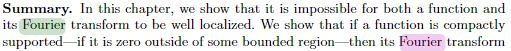
\includegraphics[width=\linewidth]{implementation/example_pdf.jpg}
  \caption{Rendered PDF Snippet}
  \label{fig:sfig:pdf_snippet}
  \end{subfigure}
  
  \begin{subfigure}{.9\textwidth}
  \centering
  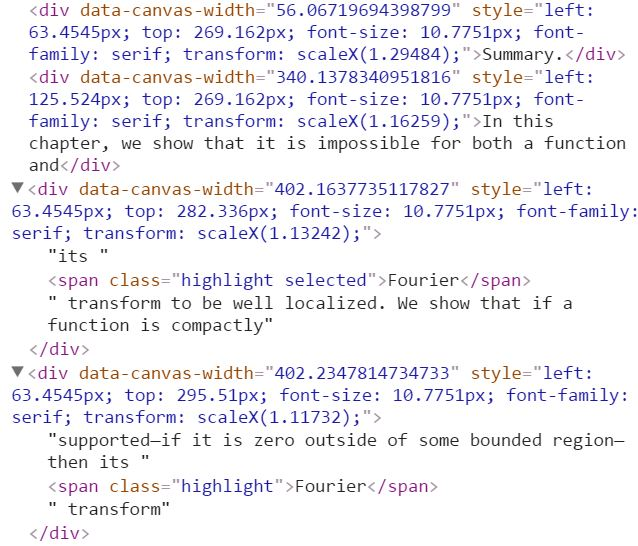
\includegraphics[width=\linewidth]{implementation/example_text_layer.jpg}
  \caption{Text Layer of the PDF Snippet}
  \label{fig:sfig:text_layer}
  \end{subfigure}
 
\caption{Text Layer of Rendered PDF}
\label{fig:text_layer}
\end{figure}

Figure \ref{fig:text_layer} shows a PDF snippet rendered by PDF.js and its corresponding text layer. As seen, each \texttt{div} is rendered with a specific position to overlay the underlying layer. The two occurrences of the highlighted term \enquote{Fourier} are both enclosed by \texttt{<span>} tag and have CSS classes. Both CSS classes \texttt{highlight} and \texttt{select} have an attribute \texttt{background-color} to specify the span's background. Therefore, terms in a PDF document can be highlighted by enclosing each term with \texttt{<span>} tag and adding a CSS class to specify the background color.

To locate an exact term in a document given the \textit{n}-th match, jQuery's \texttt{find()} function can be used. Below is the code snippet from \path{myfyp/dsp_search/static/dsp_search/js/details_page.js}. This jQuery statement finds the \textit{n}-th occurrence of a term and enclose it with \texttt{<span>} tag, along with some necessary attributes.

\begin{minted}{js}
  $pdf_viewer
      .find("#viewer .textLayer > div:icontains('" + term + "')")
      .each(function() {
        var matches = getImatchIndexes($(this).text(), term);

        for (var i = 0; i < matches.length; i++) {
          count++;
          if (nth_match.indexOf(count) > -1) {
            var text = $(this).text(),
                $span = $("<span></span>"),
                cname = $(".tree li a[data-concept-label='" + 
                    concept_label + "']").text();
            $span.attr({
              "data-concept-label": concept_label,
              "title": "Concept: " + cname
            });
            if (show_highlight) {
              $span.addClass("highlight mapping");
            }
            $span.text(term);
            $(this).html(text.substr(0, matches[i]) + 
                $span[0].outerHTML + 
                text.substr(matches[i] + term.length));
          }
        }
      });
\end{minted}
